%\documentclass[a4paper,11pt]{article}
%\usepackage[a4paper]{}
%\usepackage[utf8]{inputenc}
%\usepackage{listings}
%\usepackage{graphicx}
%\begin{document}

\section{Sensorenhet}
Sensorenheten har till uppgift att läsa in data från robotens sensorer, tolka den och vidarebefodra den till huvudenheten. En reflexsensormodul används för att roboten skall kunna hålla sig på banan. För att kunna detektera paket kommer roboten ha en avståndssensor på vardera sida. \\

\begin{figure}[h]
\center
\scalebox{0.9}{% Graphic for TeX using PGF
% Title: /home/kebabdjuret/Documents/skola/tsea29/gloria/dokumentation/designspecifikation/sensorenhet-blockschema.dia
% Creator: Dia v0.97.2
% CreationDate: Thu Oct  9 14:42:10 2014
% For: kebabdjuret
% \usepackage{tikz}
% The following commands are not supported in PSTricks at present
% We define them conditionally, so when they are implemented,
% this pgf file will use them.
\ifx\du\undefined
  \newlength{\du}
\fi
\setlength{\du}{15\unitlength}
\begin{tikzpicture}
\pgftransformxscale{1.000000}
\pgftransformyscale{-1.000000}
\definecolor{dialinecolor}{rgb}{0.000000, 0.000000, 0.000000}
\pgfsetstrokecolor{dialinecolor}
\definecolor{dialinecolor}{rgb}{1.000000, 1.000000, 1.000000}
\pgfsetfillcolor{dialinecolor}
\pgfsetlinewidth{0.100000\du}
\pgfsetdash{}{0pt}
\pgfsetdash{}{0pt}
\pgfsetmiterjoin
\definecolor{dialinecolor}{rgb}{1.000000, 1.000000, 1.000000}
\pgfsetfillcolor{dialinecolor}
\fill (15.427300\du,9.486540\du)--(15.427300\du,17.645911\du)--(20.127300\du,17.645911\du)--(20.127300\du,9.486540\du)--cycle;
\definecolor{dialinecolor}{rgb}{0.000000, 0.000000, 0.000000}
\pgfsetstrokecolor{dialinecolor}
\draw (15.427300\du,9.486540\du)--(15.427300\du,17.645911\du)--(20.127300\du,17.645911\du)--(20.127300\du,9.486540\du)--cycle;
\pgfsetlinewidth{0.100000\du}
\pgfsetdash{}{0pt}
\pgfsetdash{}{0pt}
\pgfsetmiterjoin
\definecolor{dialinecolor}{rgb}{1.000000, 1.000000, 1.000000}
\pgfsetfillcolor{dialinecolor}
\fill (25.040900\du,10.114600\du)--(25.040900\du,12.022980\du)--(33.816769\du,12.022980\du)--(33.816769\du,10.114600\du)--cycle;
\definecolor{dialinecolor}{rgb}{0.000000, 0.000000, 0.000000}
\pgfsetstrokecolor{dialinecolor}
\draw (25.040900\du,10.114600\du)--(25.040900\du,12.022980\du)--(33.816769\du,12.022980\du)--(33.816769\du,10.114600\du)--cycle;
\pgfsetlinewidth{0.100000\du}
\pgfsetdash{}{0pt}
\pgfsetdash{}{0pt}
\pgfsetmiterjoin
\definecolor{dialinecolor}{rgb}{1.000000, 1.000000, 1.000000}
\pgfsetfillcolor{dialinecolor}
\fill (25.039100\du,12.551500\du)--(25.039100\du,14.459880\du)--(33.816769\du,14.459880\du)--(33.816769\du,12.551500\du)--cycle;
\definecolor{dialinecolor}{rgb}{0.000000, 0.000000, 0.000000}
\pgfsetstrokecolor{dialinecolor}
\draw (25.039100\du,12.551500\du)--(25.039100\du,14.459880\du)--(33.816769\du,14.459880\du)--(33.816769\du,12.551500\du)--cycle;
\pgfsetlinewidth{0.100000\du}
\pgfsetdash{}{0pt}
\pgfsetdash{}{0pt}
\pgfsetbuttcap
{
\definecolor{dialinecolor}{rgb}{0.000000, 0.000000, 0.000000}
\pgfsetfillcolor{dialinecolor}
% was here!!!
\pgfsetarrowsend{to}
\definecolor{dialinecolor}{rgb}{0.000000, 0.000000, 0.000000}
\pgfsetstrokecolor{dialinecolor}
\draw (25.040900\du,11.068790\du)--(20.106300\du,11.102900\du);
}
\pgfsetlinewidth{0.100000\du}
\pgfsetdash{}{0pt}
\pgfsetdash{}{0pt}
\pgfsetbuttcap
{
\definecolor{dialinecolor}{rgb}{0.000000, 0.000000, 0.000000}
\pgfsetfillcolor{dialinecolor}
% was here!!!
\pgfsetarrowsend{to}
\definecolor{dialinecolor}{rgb}{0.000000, 0.000000, 0.000000}
\pgfsetstrokecolor{dialinecolor}
\draw (25.039100\du,13.505690\du)--(20.077600\du,13.540100\du);
}
% setfont left to latex
\definecolor{dialinecolor}{rgb}{0.000000, 0.000000, 0.000000}
\pgfsetstrokecolor{dialinecolor}
\node[anchor=west] at (17.189200\du,13.801900\du){AVR};
\pgfsetlinewidth{0.100000\du}
\pgfsetdash{}{0pt}
\pgfsetdash{}{0pt}
\pgfsetbuttcap
{
\definecolor{dialinecolor}{rgb}{0.000000, 0.000000, 0.000000}
\pgfsetfillcolor{dialinecolor}
% was here!!!
\pgfsetarrowsstart{to}
\pgfsetarrowsend{to}
\definecolor{dialinecolor}{rgb}{0.000000, 0.000000, 0.000000}
\pgfsetstrokecolor{dialinecolor}
\draw (11.216500\du,13.588400\du)--(15.427300\du,13.566200\du);
}
\pgfsetlinewidth{0.100000\du}
\pgfsetdash{}{0pt}
\pgfsetdash{}{0pt}
\pgfsetmiterjoin
\definecolor{dialinecolor}{rgb}{1.000000, 1.000000, 1.000000}
\pgfsetfillcolor{dialinecolor}
\fill (6.691550\du,13.088400\du)--(6.691550\du,14.088391\du)--(11.216510\du,14.088391\du)--(11.216510\du,13.088400\du)--cycle;
\definecolor{dialinecolor}{rgb}{0.000000, 0.000000, 0.000000}
\pgfsetstrokecolor{dialinecolor}
\draw (6.691550\du,13.088400\du)--(6.691550\du,14.088391\du)--(11.216510\du,14.088391\du)--(11.216510\du,13.088400\du)--cycle;
% setfont left to latex
\definecolor{dialinecolor}{rgb}{0.000000, 0.000000, 0.000000}
\pgfsetstrokecolor{dialinecolor}
\node[anchor=west] at (7.016550\du,13.788400\du){Huvudenhet};
% setfont left to latex
\definecolor{dialinecolor}{rgb}{0.000000, 0.000000, 0.000000}
\pgfsetstrokecolor{dialinecolor}
\node[anchor=west] at (12.814700\du,13.430700\du){SPI};
\pgfsetlinewidth{0.100000\du}
\pgfsetdash{}{0pt}
\pgfsetdash{}{0pt}
\pgfsetbuttcap
{
\definecolor{dialinecolor}{rgb}{0.000000, 0.000000, 0.000000}
\pgfsetfillcolor{dialinecolor}
% was here!!!
\pgfsetarrowsend{to}
\definecolor{dialinecolor}{rgb}{0.000000, 0.000000, 0.000000}
\pgfsetstrokecolor{dialinecolor}
\draw (17.799700\du,20.290500\du)--(17.777300\du,17.645900\du);
}
% setfont left to latex
\definecolor{dialinecolor}{rgb}{0.000000, 0.000000, 0.000000}
\pgfsetstrokecolor{dialinecolor}
\node[anchor=west] at (17.099700\du,20.965500\du){JTAG};
% setfont left to latex
\definecolor{dialinecolor}{rgb}{0.000000, 0.000000, 0.000000}
\pgfsetstrokecolor{dialinecolor}
\node[anchor=west] at (21.691337\du,10.613944\du){Analog};
% setfont left to latex
\definecolor{dialinecolor}{rgb}{0.000000, 0.000000, 0.000000}
\pgfsetstrokecolor{dialinecolor}
\node[anchor=west] at (21.727000\du,13.001822\du){Analog};
% setfont left to latex
\definecolor{dialinecolor}{rgb}{0.000000, 0.000000, 0.000000}
\pgfsetstrokecolor{dialinecolor}
\node[anchor=west] at (29.428835\du,11.068790\du){};
% setfont left to latex
\definecolor{dialinecolor}{rgb}{0.000000, 0.000000, 0.000000}
\pgfsetstrokecolor{dialinecolor}
\node[anchor=west] at (25.581850\du,11.132679\du){Vänster avståndssensor};
% setfont left to latex
\definecolor{dialinecolor}{rgb}{0.000000, 0.000000, 0.000000}
\pgfsetstrokecolor{dialinecolor}
\node[anchor=west] at (25.841217\du,13.629092\du){Höger avståndssensor};
\pgfsetlinewidth{0.100000\du}
\pgfsetdash{}{0pt}
\pgfsetdash{}{0pt}
\pgfsetmiterjoin
\definecolor{dialinecolor}{rgb}{1.000000, 1.000000, 1.000000}
\pgfsetfillcolor{dialinecolor}
\fill (24.998273\du,15.152876\du)--(24.998273\du,17.065712\du)--(33.849190\du,17.065712\du)--(33.849190\du,15.152876\du)--cycle;
\definecolor{dialinecolor}{rgb}{0.000000, 0.000000, 0.000000}
\pgfsetstrokecolor{dialinecolor}
\draw (24.998273\du,15.152876\du)--(24.998273\du,17.065712\du)--(33.849190\du,17.065712\du)--(33.849190\du,15.152876\du)--cycle;
% setfont left to latex
\definecolor{dialinecolor}{rgb}{0.000000, 0.000000, 0.000000}
\pgfsetstrokecolor{dialinecolor}
\node[anchor=west] at (29.423732\du,16.109294\du){  };
\pgfsetlinewidth{0.100000\du}
\pgfsetdash{}{0pt}
\pgfsetdash{}{0pt}
\pgfsetbuttcap
{
\definecolor{dialinecolor}{rgb}{0.000000, 0.000000, 0.000000}
\pgfsetfillcolor{dialinecolor}
% was here!!!
\pgfsetarrowsend{to}
\definecolor{dialinecolor}{rgb}{0.000000, 0.000000, 0.000000}
\pgfsetstrokecolor{dialinecolor}
\draw (24.998273\du,16.109294\du)--(20.135132\du,16.125505\du);
}
% setfont left to latex
\definecolor{dialinecolor}{rgb}{0.000000, 0.000000, 0.000000}
\pgfsetstrokecolor{dialinecolor}
\node[anchor=west] at (21.629737\du,15.530656\du){Analog};
% setfont left to latex
\definecolor{dialinecolor}{rgb}{0.000000, 0.000000, 0.000000}
\pgfsetstrokecolor{dialinecolor}
\node[anchor=west] at (27.429844\du,16.255188\du){Reflexsensor};
\end{tikzpicture}
}
\caption{Blockschema över sensorenheten}
\end{figure}

\subsection{Reflexsensormodul}
Reflexsensormodulen består av 11 reflexsensorer. En reflexsensor består av en lysdiod och en fototransistor. Fototransistorn har ett analogt utvärde mellan 0 och 5V beroende på hur mycket ljus som fångas upp. Genom att sätta enable för en lysdiod till 1 och sedan läsa av den tillhörande fototransistorn kan vi avgöra om underlaget är ljust eller mörkt. Fototransistorn läses av med en AD-omvandling på AVRen. Detta görs för varje reflexsensor och på så sätt kan vi detektera tejpens position under sensorn eftersom tejpen banan består av får förutsättas ha en annan färg än golvet. Eftersom AVRen har ett begränsat antal pinnar med AD-omvandling, muxar vi fototransistorernas utgångar till en enda pinne på AVRen. Då vi inte vill ha mer än en lysdiod igång samtidigt kommer vi använda ytterligare en mux för att styra en enablesignal till den lysdiod vi vill använda, övriga kommer vara avslagna.

\subsubsection{Kalibrering}
Beroende på vilket underlag roboten arbetar på kommer värdena för golv och tejp att variera. Vi behöver därför kunna kalibrera sensorn för att sätta standardvärden. Detta kommer ske på ett sådant sätt att vi först låter roboten titta på bara golvet och sedan en bit tejp. Vi sparar de värden vi får under dessa testfall och använder dem som referens när vi ska detektera golv eller tejp.

\subsection{Avståndssensor}
För att kunna detektera paket kommer roboten ha en avståndssensor på höger respektive vänster sida. Dessa kommer vara av typen GP2D120 och använder IR för att generera en analog signal. Denna signal läses av med en AD-omvandling på AVRen. Då sensorns utsignal är olinjär kommer vi under utveckligsfasen ta fram en tabell med närmevärden för olika distanser. Utsignalen jämförs med denna tabell för att estimera det uppmätta avståndet till ett föremål.

\subsection{Mjukvara}
Sensorenheten kör kontinuerligt en loop där den läser och lagrar data från sensorerna. Då huvudenheten skickar en instruktion till sensorenheten körs en avbrottsrutin där instruktionen tolkas och utförs. Antingen kalibreras sensorerna eller så returnerar sensorenheten data för den adresserade sensorn.

%Figur \ref{systemskiss:sensorschema} visar flödesschema över mjukvaran i sensormodulen.

%\begin{figure}[h]
%\center
%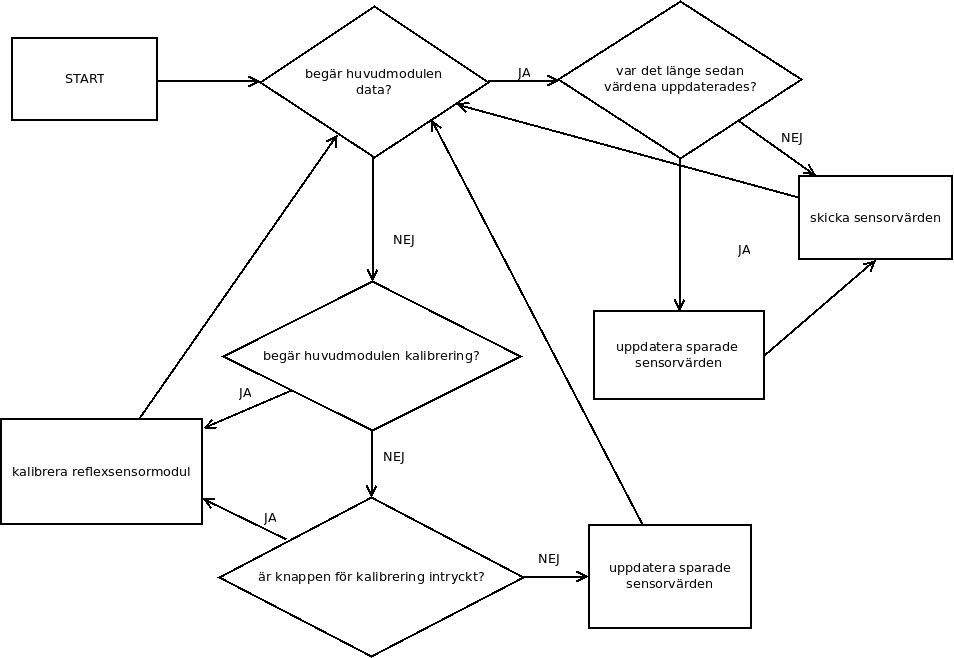
\includegraphics[scale=0.4]{sensorflow}
%\caption{Flödesschema för sensormodul.} \label{systemskiss:sensorschema}
%\end{figure}

%\todo{Nya flödescheman för sensorenhet. Avbrottsrutiner osv.}

%\end{document}

\subsection{Komponenter}
Följande komponenter är nödvändiga för konstruktion av sensorenheten. \\

\begin{tabularx}{\textwidth}{| l | X |}
	\hline
	{\textbf{Komponent}} & {\textbf{Tillgänglighet}} \\\hline
	{En AVR av typ Atmega1284} & {Tillgänglig} \\\hline
	{En JTAG Ice 3} & {Tillgänglig} \\\hline
	{En Reflexsensormodul} & {Tillgänglig} \\\hline
	{Två muxar av typ MC14067B} & {Tillgängliga} \\\hline
	{Två avsåndssensorer av typ GP2D120} & {Tillgängliga} \\\hline
	{En avstudsad tryckknapp} & {Tillgänglig} \\\hline
\end{tabularx}
